\section{CKAN}
\label{sec:ckan}

The Comprehensive Knowledge Archive Network, or CKAN\footnote{\url{https://ckan.org/}}, is an open source\footnote{\url{https://github.com/ckan/ckan}} data management system. In particular, CKAN is the world's leading tool for making Open Data websites, helping to manage and publish collections of data. It is mainly used by national and local governments, research institutions and other organizations who collect data. Two examples are the U.S. Government's Open Data portal, shown in Figure \ref{fig:ckan-usa} or the Roma Capitale's Open Data portal, shown in Figure \ref{fig:ckan-roma}.

\begin{figure}[!ht]
  \begin{subfigure}{.5\columnwidth}
    \centering
    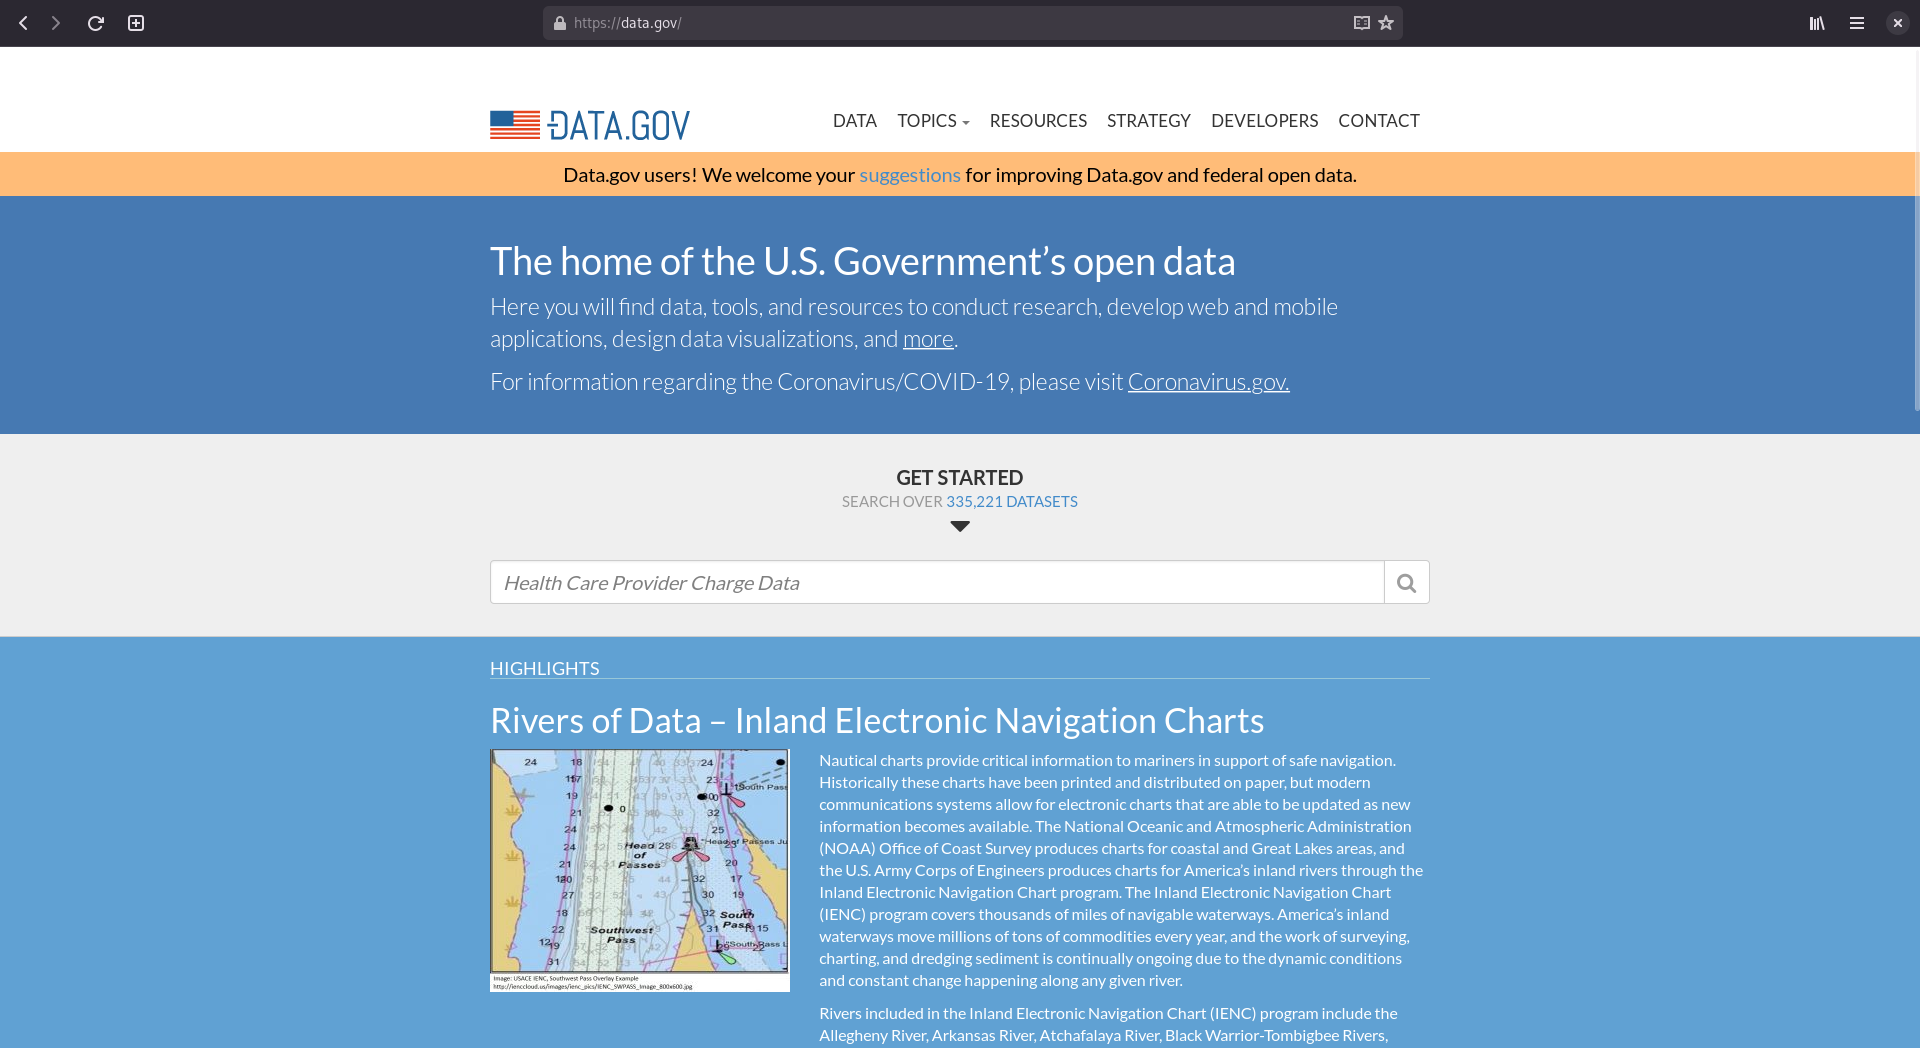
\includegraphics[width=.99\linewidth]{images/ckan/ckan-usa}
    \subcaption{U.S. Government's Open Data portal.\footnote{\url{https://data.gov/}}}
    \label{fig:ckan-usa}
  \end{subfigure}%
  \begin{subfigure}{.5\columnwidth}
    \centering
    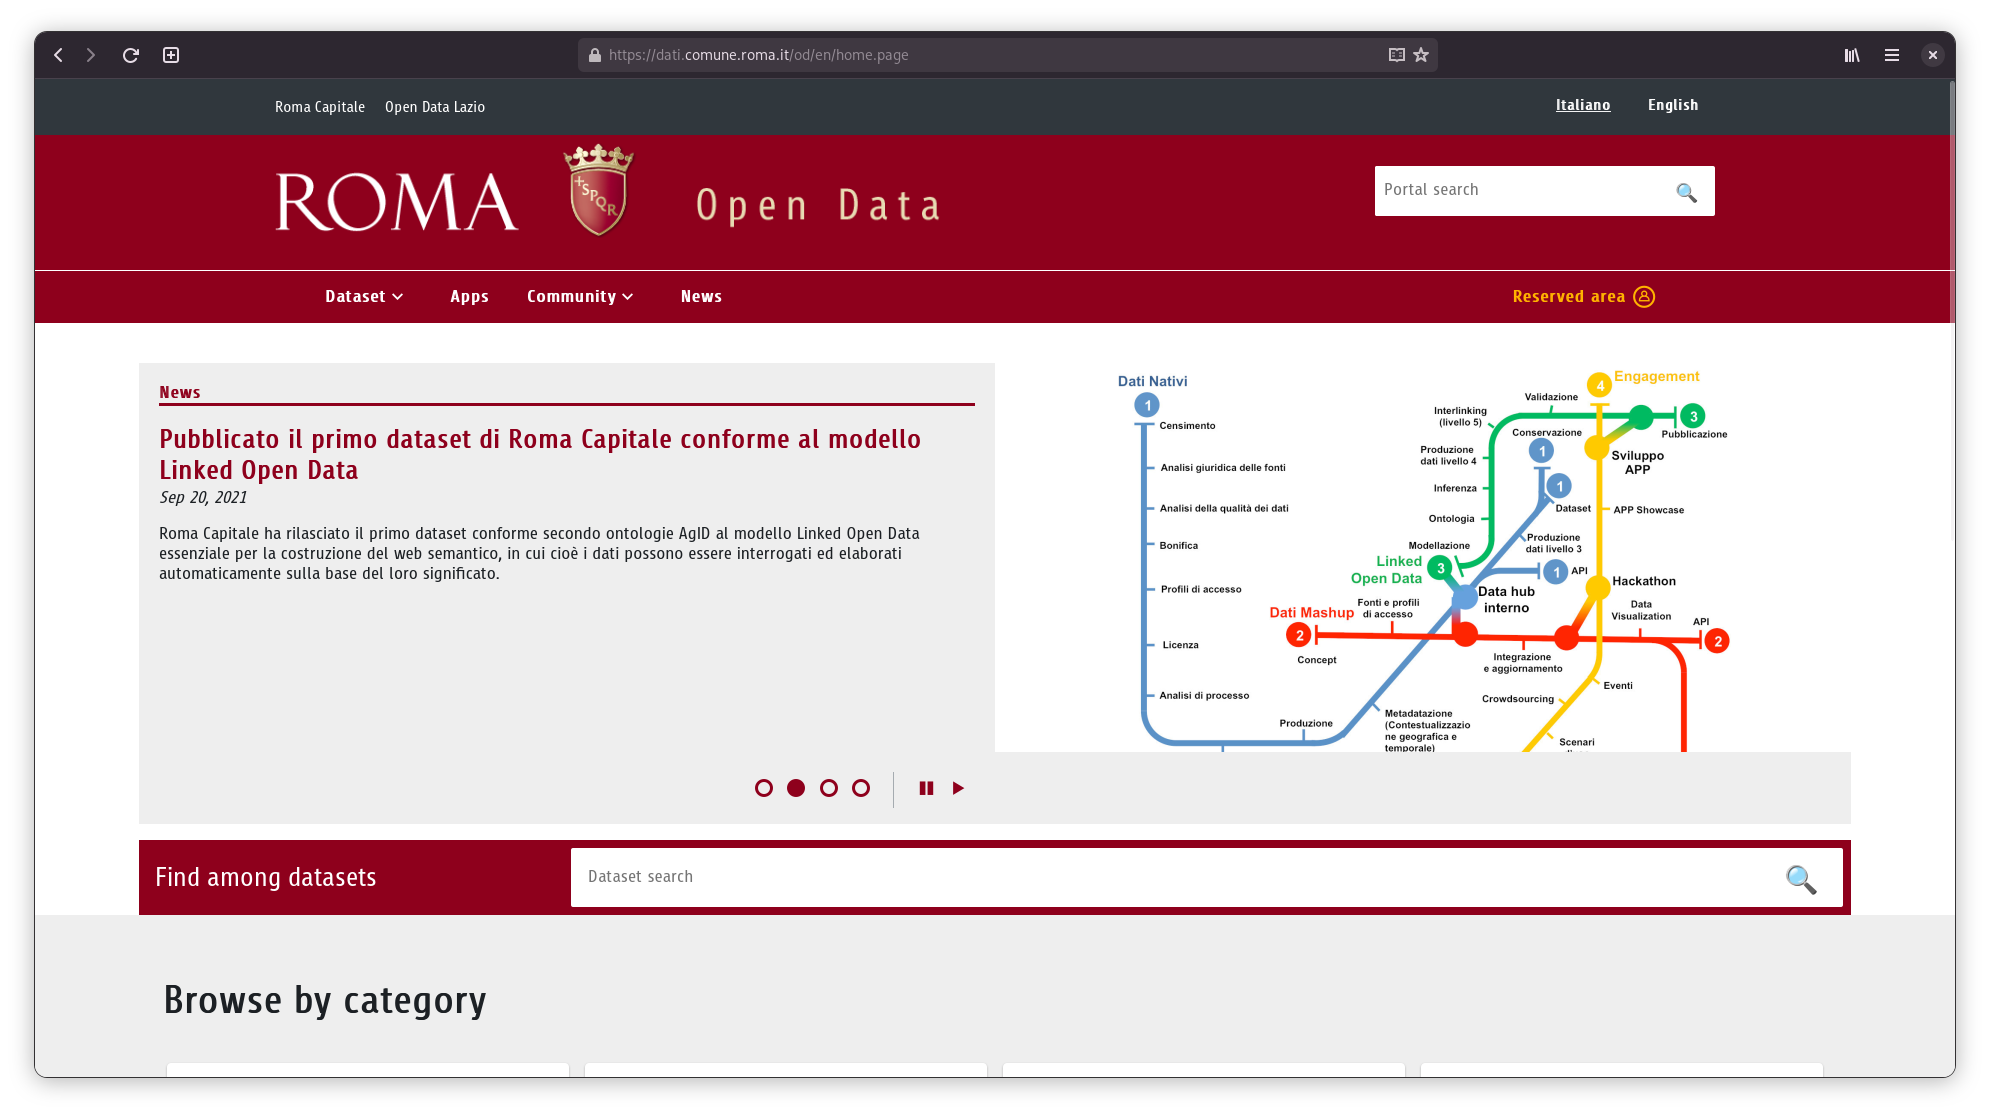
\includegraphics[width=.99\linewidth]{images/ckan/ckan-roma}
    \subcaption{Roma Capitale's Open Data portal.\footnote{\url{https://dati.comune.roma.it/}}}
    \label{fig:ckan-roma}
  \end{subfigure}
  \caption{Examples of CKAN Open Data governments portals.}
  \label{fig:ckan-examples}
\end{figure}

In CKAN data is published in units called \textit{datasets}. Each dataset is owned by an \textit{organization} and contains information about the data like the title, publisher, data or the license; and one or more resources which are the data itself. For example, a dataset can contain different files, like the data for different years, or the same data in different formats. Any user can view, download, and search for public datasets, but there is also the possibility to restrict the access of some datasets only for registered and authorized users.

Despite the core version of CKAN has only few basic features, one of the strengths of this tool is the possibility to add different plugins which extend its functionalities and customize the user interface. The most popular plugins, developed and maintained by CKAN itself, are: (1) different tools to visualize data directly on the web page, such as tables, plots or maps; (2) DataStore extension that provides an \textit{ad hoc} database for storage of structured data from resources and integrates them into CKAN \acs{API} to return data in \ac{JSON} format; (3) DCAT extension that includes \ac{RDF} serialization of datasets and harvesters to import \ac{RDF} resources into CKAN. An example of this feature can be seen in the Italian Open Data portal\footnote{\url{https://www.dati.gov.it/}}, that include the datasets from all the local governments.